\section{Introduction}

% Motivate need for new process
The Haber-Bosch process for thermochemical synthesis of ammonia from nitrogen and hydrogen transformed the global fertilizer industry and is a critical enabler of the continued expansion of human populations \cite{Smil_1999}. The process is an impressive feat of modern chemical engineering, producing around 150 million tons of ammonia per year at a thermodynamic efficiency of up to 70\% \cite{Schloegl_2003,Schiffer_2017}. However, the process also has downsides. The scale of the process leads to massive energy consumption of 2.5 exajoule per year, and the hydrogen feedstock is typically obtained via methane reforming, leading to a carbon footprint of 340 Mt of CO$_2$ equivalent per year; this is the highest impact of any commodity chemical \cite{Schiffer_2017}. Furthermore, the high temperatures ($\sim$700 K) and pressures ($\sim$100 bar) lead to substantial capital cost and economies of scale, driving highly centralized production. This is in contrast to the decentralized use of ammonia-based fertilizers (Fig. \ref{fig:usemap}), which results in high transportation costs and additional emissions \cite{West_2002}. This is particularly impactful in remote locations such as sub-Saharan Africa, where soils are often nutrient-limited due to lack of access to fertilizers \cite{Gilbert_2012, Mueller_2012}. The opposite problem of over-fertilization also has a negative environmental impact in more developed nations due to the periodic application of highly concentrated fertilizers that cause nitrate pollution in waterways and vast ocean ``dead zones'' through leaching \cite{Diaz2008}. Finally, the intense conditions and reactive nature of concentrated ammonia based fertilizers lead to safety and national security concerns, as evidenced by explosions at fertilizer plants and the common use of fertilizers in makeshift explosives \cite{Marlair_2005}.

%\begin{figure}
%    \centering
%    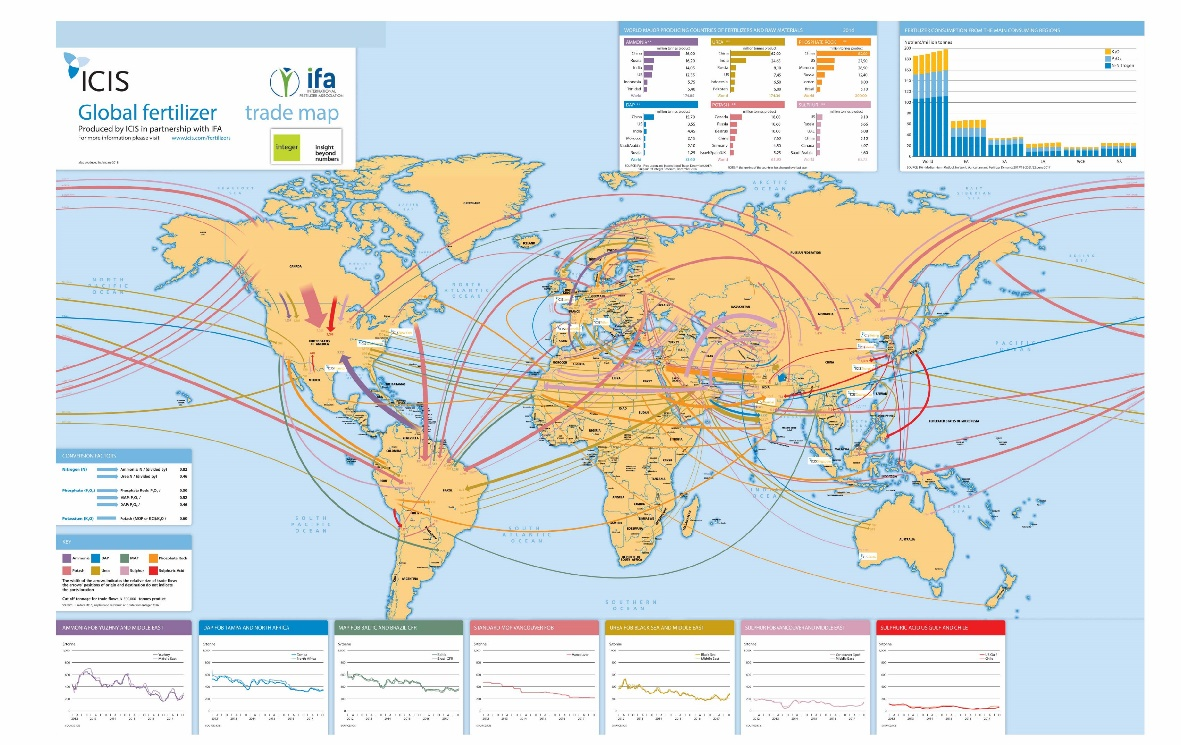
\includegraphics[width=1\textwidth]{Figures/decentralization.jpg}
%    \caption{\hl{placeholder figure for illustration of decentralization. Overlay fertilizer use with locations of ammonia plants. Possibly include solar flux map.}}
%    \label{fig:usemap}
%\end{figure}

\begin{figure}
    \centering
    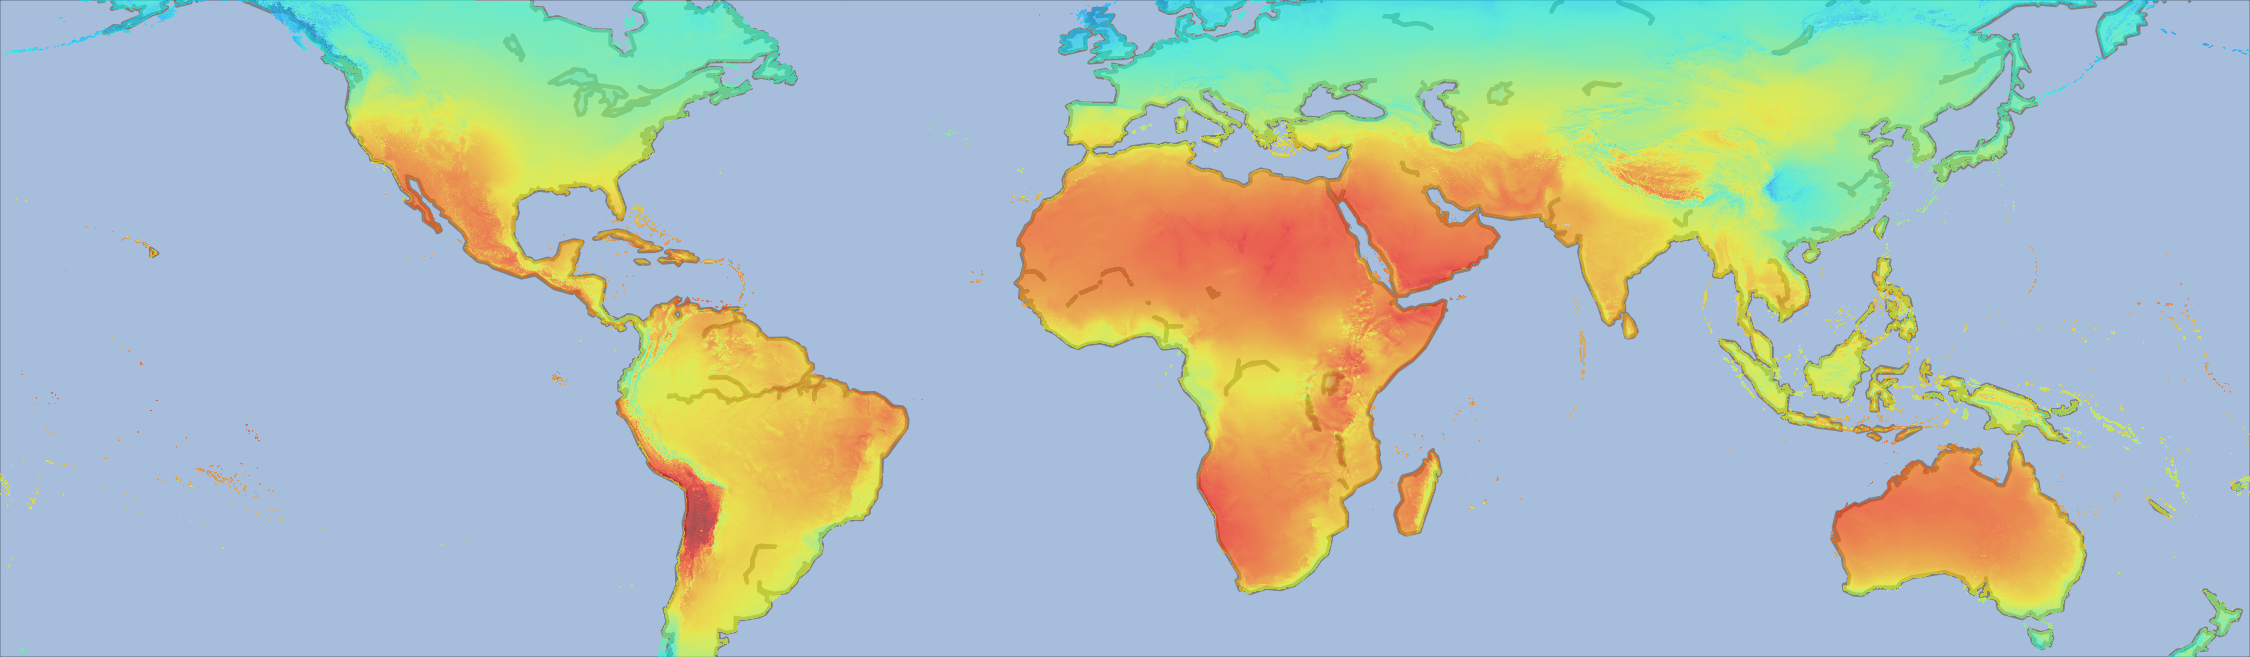
\includegraphics[width=1\textwidth]{Figures/solar_map.png}
    %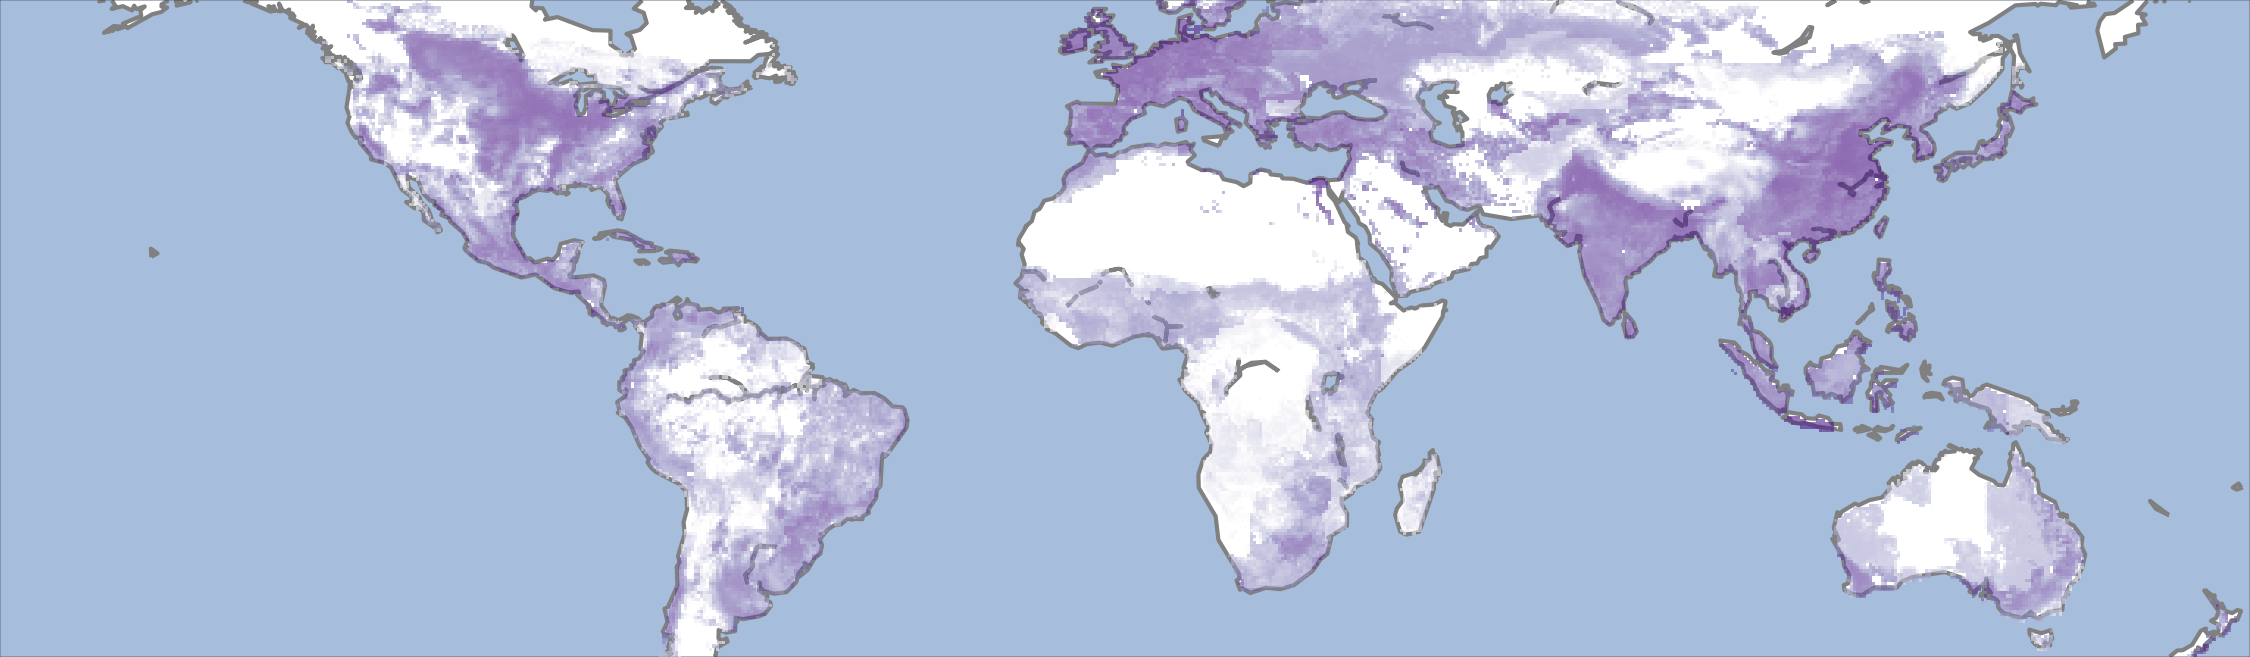
\includegraphics[width=1\textwidth]{Figures/N_fertilizer_map.png}
    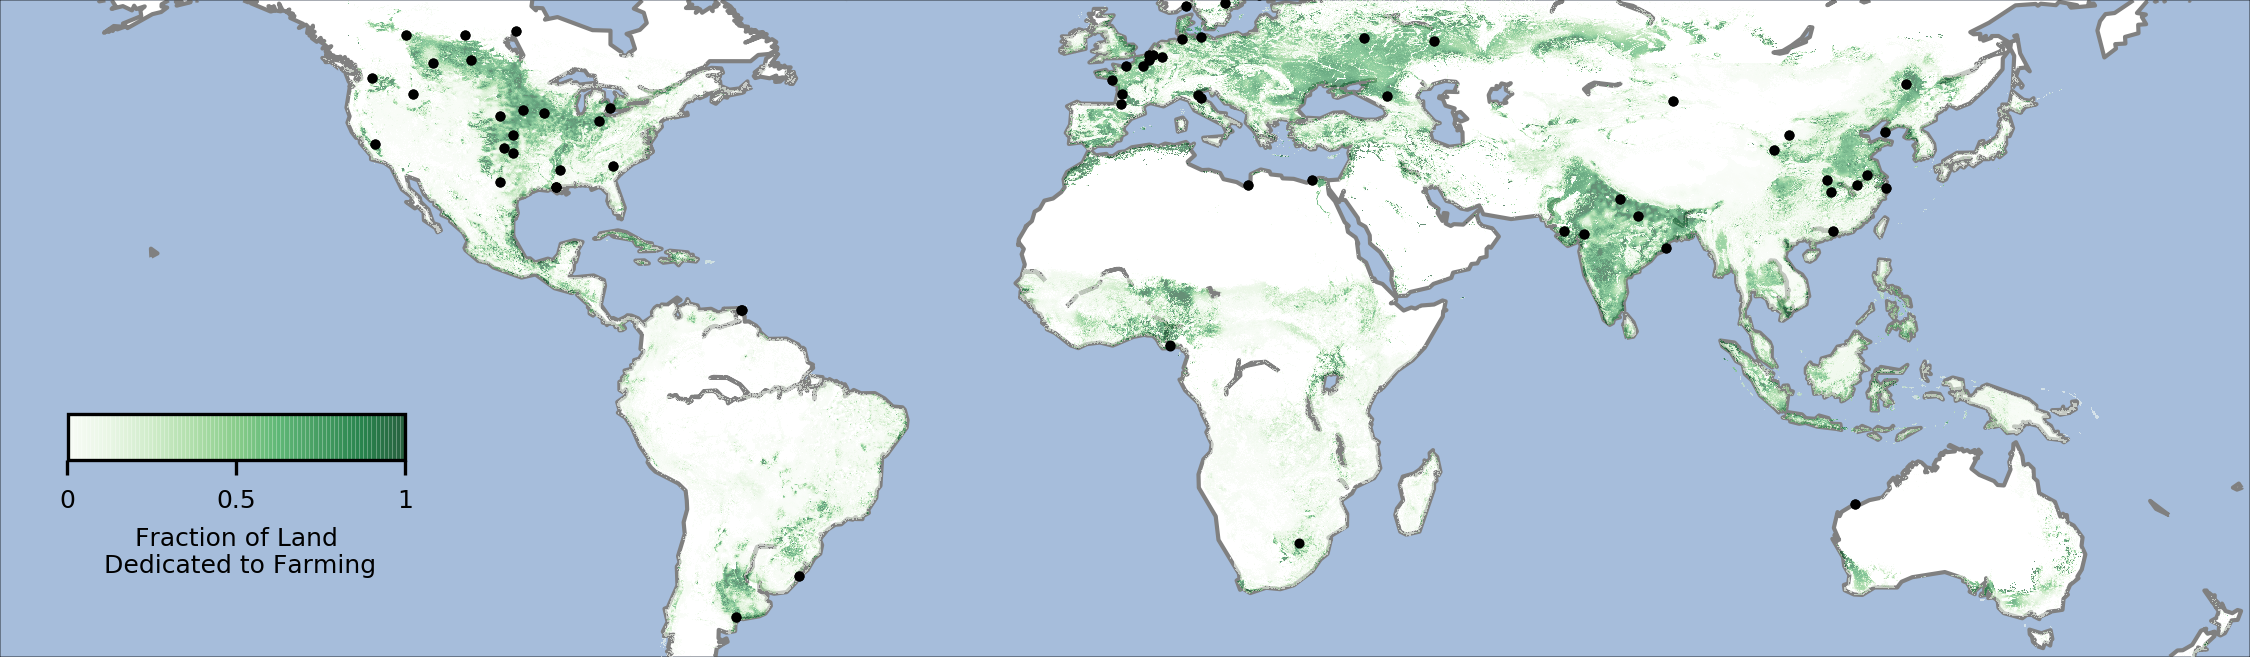
\includegraphics[width=1\textwidth]{Figures/croplands_map.png}
    \caption{(top)Horizontal solar radiation intensity over the surface of the earth averaged ($kW/m^2$) (bottom) percent of land dedicated to crop production (\%)}
    \label{fig:usemap}
\end{figure}

%http://sedac.ciesin.columbia.edu/data/sets/browse?facets=theme:agriculture
%http://globalsolaratlas.info/downloads/world

% Motivate solar fertilizers
One possible strategy to overcome these disadvantages is decentralized production of fertilizers using solar energy. These ``solar fertilizers'' provide a route to harness solar energy, nitrogen, and water/oxygen from the air to produce lower-concentration ammonia- or nitrate-based fertilizers at or near the point of use. This is advantageous from the perspective of solar energy capture since the intermittent energy is directly captured in a storable product that can be utilized near the point of production, avoiding issues with electricity storage and transport \cite{MacKay_2013}. There are also advantages from an agricultural perspective, since inexpensive feedstocks and reduced transport costs may significantly improve access to fertilizers in remote and developing regions, and the use of lower-concentration fertilizers may enable novel strategies of nutrient management that can reduce groundwater pollution. Further, low-concentration fertilizers produced at ambient conditions are inherently safer both from the perspective of the process and the product. Although fertilizers require a range of nutrients including N, P, and K, we focus on N fertilizers in this work since it is often the limiting nutrient\cite{Yousaf2017}. Additionally, in developing regions such as Africa, there exists an overabundance of soil P fertilization with respect to N\cite{VanderVelde2014}, limiting crop productivity. %and the production is the most centralized (I think this statement is false, ) \needcite.% the key challenge lies in the fixation of nitrogen and hence this work is focused solely on nitrogen-based fertilizers. 
%Development of solar-driven nitrogen fixation would likely serve as a driver for the development of solar technologies for other nutrients.
%\hl{This is a little awkward, but we need to point out somewhere that we are only considering N2 fixation here. I'm not sure we even need to address the P and K fertilizers. mch- I think this is OK, the last sentence regarding motivating other solar nutrient technologies might not be needed though}

% Motivate need for collaboration with agriculture/fertilizer
Solar fertilizers hold substantial promise as a route to solar energy capture and sustainable agriculture, but there are also considerable challenges. One critical challenge is in the development of a viable strategy for efficiently using solar energy to dissociate the strong dinitrogen triple bond at ambient conditions. Nitrogen fixation at ambient conditions is a key objective of chemistry, and has been the subject of considerable research in homogeneous catalysis, enzyme catalysis, and bioengineering, yet no viable strategies have emerged due to issues with low conversion and/or stability under realistic conditions \cite{Vicente_2017,Bur_n_2017,MacLeod_2013,Foster2018}. %need more citations here.
More recently there has been a surge of interest in photo- and electrocatalytic nitrogen fixation by heterogeneous catalysts \cite{Medford_2017,Kyriakou_2017,Foster_2018,Chen_2018}. This route is particularly interesting from the perspective of solar fertilizers since photoelectrochemical systems interface well with solar energy, have the potential to scale relatively easily, and have been the subject of considerable research in the solar fuels community \cite{Kondratenko2013}. However, further work is needed to improve the yield and efficiency of photo- and electrochemical nitrogen fixation. %In this work we focus on photo(electro)chemical routes to solar fertilizer production and seek to identify targets and strategies for future research.

Solar fertilizers are also expected to differ significantly from traditional fertilizers, opening a range of additional agronomic challenges and opportunities. One key difference is that solar fertilizers are expected to have considerably lower fixed nitrogen concentrations, owing to the fact that photo(electro)chemical nitrogen fixation efficiencies are unlikely to compete with the 70\% efficiency of the Haber-Bosch process \cite{Schloegl_2003, Singh_2017}. %cite selectivity challenge papers?
Separating and concentrating the ammonia will require additional steps that add complexity to the process and require energy. Direct utilization of dilute fertilizers will avoid or reduce the amount of energy needed for separation/concentration, and may also enable more controlled nutrient management. However, this represents a paradigm shift in agricultural practice, and considerable effort is needed to understand how dilute solar fertilizers can be sustainably and practically integrated with agricultural systems. These considerations will also inform the development of the photo(electro)catalytic processes for solar fertilizer production, and hence should be considered in parallel.

In this work we identify key considerations and performance targets for the photo(electro)chemical production of dilute solar fertilizers from the perspective of catalysis and agronomics. Some specific advantages and disadvantages of dilute and decentralized fertilizer production are outlined and the potential agronomic use cases and impacts are examined. Some specific strategies for the design of a reaction/separation process for photo(electro)chemical fertilizer production are considered, and assessed qualitatively on the bases of metrics that will impact their ultimate viability. These possible designs are used along with back-of-the-envelope calculations to quantify initial performance targets and limiting cases for catalyst reactivity and separation efficiency and suggest specific materials properties and tests that will inform process design. We hope that these considerations will serve as a foundation and guide for future research in the development of photo(electro)chemical processes for solar fertilizer production.

\section{Agronomics of solar fertilizers}

\subsection{Decentralization of fertilizer production}
\label{sec:decentralized}

Current fertilizer production relies on the Haber-Bosch process, which is highly centralized with fewer than 100 total production plants \cite{McArthur_2017} for over 500 million total farms \cite{FAO_2014,Lowder_2016}. The centralization is driven primarily by the harsh reaction conditions of the process. The high temperature ($\sim$450 $^\circ$ C) and particularly pressure ($\sim$ 20 bar) of the process lead to a favorable economy of scale, with a typical scaling factor of 0.7 \cite{Ullmann_amm_2006}. This incentivizes high-volume production and high capital investment, with most plants operating at a capacity greater than 1200 tonne day$^-1$ with a typical capital cost of \hl{???} \cite{Ullmann_amm_2006}. This leads to long payback periods, and encourages development of production facilities in regions with stable access to the natural gas feedstock and reliable infrastructure \cite{McArthur_2017}, as indicated by the presence of ammonia production primarily in the developed world (see Fig. \ref{fig:map}). This section briefly explores the implications of the centralized Haber-Bosch process on the economics of fertilizer production, and explores the potential impact and challenges of decentralized fertilizer in the developed and developing worlds.

The price and price volatility of fertilizer is controlled by a complex interplay of geopolitical and economic factors \cite{Huang2007,Etienne2016}. A detailed analysis is beyond the scope of this work, but we briefly introduce some key concepts. The cost of fertilizers can be broken down into production, transportation, and storage. The production cost of fertilizer is controlled primarily by the cost of natural gas used to produce hydrogen for the Haber-Bosch process, and hence varies with location, economic, and geopolitical factors. 
This leads to variable and uncertain cost of fertilizers and presents challenges in agricultural planning \cite{Etienne2016}. Furthermore, the cost of transportation is highly variable depending on location. Barge, pipeline, and rail transport are normally used for long-distance anhydrous ammonia transportation, while trucks are preferred for short distances. Distance, location of plant site relative to the agricultural area, availability of transportation equipment, and relative cost of available carriers are the major governing factors for selection of a typical anhydrous ammonia transportation system. Typical costs reported for long distance (greater than 1600 km) pipeline, barge, and rail transport are \$0.0153, \$0.0161 and \$0.0215 per ton per kilometer, respectively \cite{ammonia_encyclopedia}.  Short truck transportation costs are expected to be much higher. For distances of the order of 100 km, typical costs of \$0.0365 per ton per kilometer are reported \needcite. Overall, international shipping of ammonia between the United States and Western Europe costs on the order of \$ 35/t \needcite. Additionally, storage costs must be considered due to the cyclic nature of agricultural ammonia consumption caused by the harvest seasons. It has been reported that roughly 75\% of the dedicated fertilizer production is sold during the harvest season \needcite. To reduce storage costs resulting from this cyclic consumption pattern, large refrigerated anhydrous ammonia storage vessels are used, which add another \$11-80/t to ammonia cost \cite{IFDC_1998,ammonia_encyclopedia}. Thus, the freight costs can account for more than half of the delivered cost of ammonia in some countries \needcite. The variation in ammonia production costs in different countries is presented in Figure \ref{fig:relative_costs} \cite{maxwell2004synthetic}, showing that in many regions outside the US the cost of gas feedstocks accounts for less than half of the total cost. The hazardous nature of ammonia also leads to challenges with transportation and storage, particularly in regions with poor infrastructure \cite{Etienne2016}. 

\begin{figure}
    \centering
    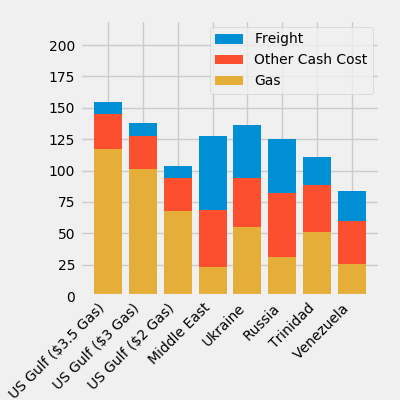
\includegraphics[width=0.5\textwidth]{Figures/Cost_By_location.png}
    \caption{Data from Maxwell 2004\cite{maxwell2004synthetic}, }
    \label{fig:relative_costs}
\end{figure}

The production, transportation, and storage costs are the main components of fertilizer price, but the overall cost is not directly derived from these categories. For example, the price of fertilizer in Thailand (\$ 287/ton) is roughly half the price of fertilizer in Mozambique (\$ 567/ton), but this difference cannot be attributed directly to any single category. One critical factor that controls this overall price is economy of scale. Developing nations in Africa are often purchasing smaller quantities of fertilizer from the international market, leading to a limited ability to bargain for lower wholesale prices \cite{Wanzala2013}. Larger agricultural markets such as Asia are able to more effectively distribute fixed costs of transportation and negotiation across more units of fertilizer, translating to lower prices at the farm scale. This scale-up is not possible in less developed markets for a variety of reasons including port capacity and poor transportation infrastructure \needcite. Political instability often compounds this problem by causing existing infrastructure to deteriorate due to lack of use\cite{Foster_2011}. Less developed markets are also subject to more uncertain demand owing to lack of access to capital by smallholder farmers and unpredictable implementation of government subsidies \needcite. Overall, these factors lead to the perverse situation in which fertilizers are most expensive in the poorest places where the need is greatest. This is a key factor in the distressing fact that despite the tremendous technological developments of the recent decades, world hunger is currently increasing with over 800 million people suffering from undernourishment as of 2016 \cite{FAO_2017}. Notably, many of these economic and geopolitical factors could be alleviated by decentralized production of dilute fertilizers from renewable resources. Lack of dependence on natural gas would reduce volatility in fertilizer production costs \cite{Etienne2016}, and producing fertilizer at or near the point of use would reduce transportation costs and reduce the price dependence on economies of scale  \cite{IFDC_1998}. Furthermore, local production would improve certainty in fertilizer availability and reduce the influence of external factors such as tariffs and subsidies. Agricultural production has also been tied to general economic prosperity, and local fertilizer manufacturing industries in developing countries could spur substantial economic growth \cite{McArthur_2017}.
%For example, transportation costs as low as \$0.0043 per ton per km for aqueous ammonia have been reported for China \cite{guo2002animal}.

\begin{figure}
    \centering
    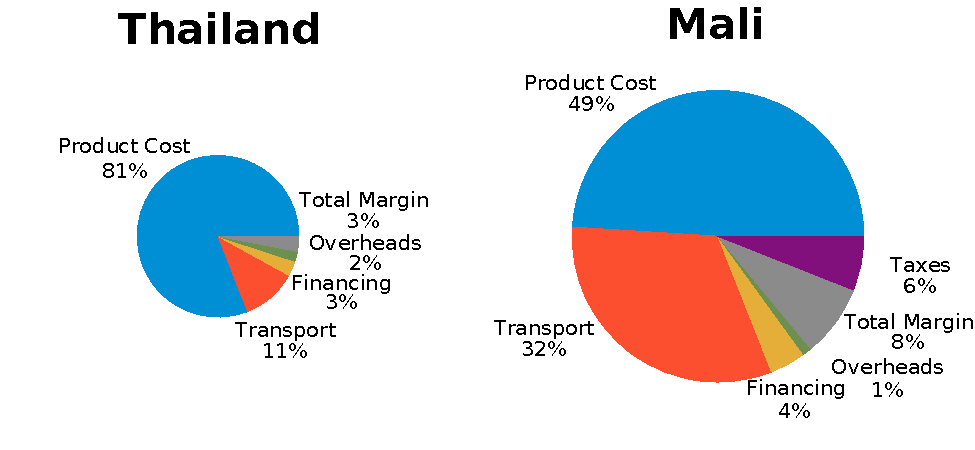
\includegraphics[width=1\textwidth]{Figures/Cost_Breakdown.pdf}
    \caption{The price breakdown for fertilizer in (a) Thailand and (b) Mali for the year 2013. Relative areas reflect the ratio of costs in the two countries (\$282 in Thailand and  \$509 in Mali) \cite{Wanzala2013} \hl{we can select different countries and/or add more. Would be interesting to include the US.}}
    \label{fig:cost_pies}
\end{figure}



%\begin{figure}
 %   \centering
 %   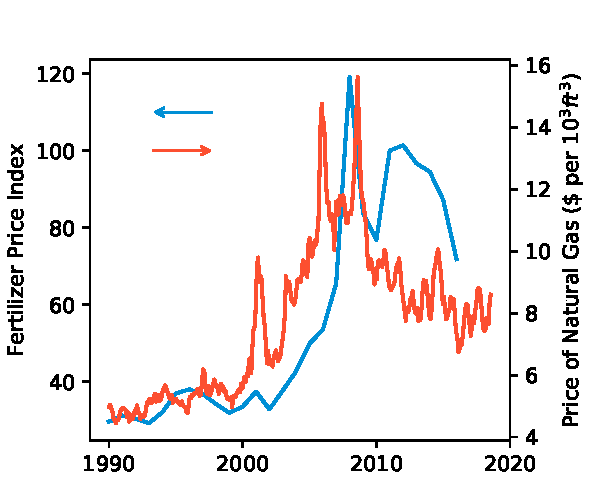
\includegraphics[width=0.7\textwidth]{Figures/gas_vs_fert.pdf}
 %   \caption{The cost of natural gas paid by industrial consumers in the United States and the price index of fertilizer between over time (www.eia.gov and usda.gov)}
%    \label{fig:gas_vs_fert}
%\end{figure}

%The concept of decentralization is difficult to quantify in general \cite{Schneider_2003}, but in this context we propose the decentralization should scale directly with the total number of fertilizer production facilities. It is useful to examine order-of-magnitude estimates of these quantities to assess the prospects of decentralization. A recent report identified a total of 63 major fertilizer production facilities based on data from the 10 largest producers of ammonia-based fertilizers \cite{McArthur_2017}. While this list may be incomplete, it is expected to be on the correct order of magnitude. A typical 1000 tpd ammonia plant can meet the ammonia requirements of many small countries. At a medium application rate of 40 kg N/ha, a typical ammonia plant can fertilize 7.5 million hectares of land. Fertilizer production on this scale is not available in many developing countries; logistics, economic and political issues constrain construction of large scale ammonia plants in such regions.\cite{IFDC_1998} 
%For landlocked countries that are located at a long distance from the ports, the freight cost doubles or even triples the cost of ammonia-based products, and thus limits consumption.

%This should be normalized by the total agricultural output, which we propose can be estimated by the total number of farms or the total amount of arable land. Both numbers are difficult to know exactly, but a 2014 report estimated the total number of farms to be in excess of 570 million with a total area of around 4.9 billion hectares (another FAO document said 1.5 billion ha) as of 2010 \cite{FAO_2014,Lowder_2016}. This indicates that a single ammonia-based fertilizer plant serves on the order of 10 million farms, or 100 million \hl{(24 million)} hectares of arable land (see Figure \ref{fig:map}) \hl{We need to refine these estimates and ensure that the 4.9 billion number does not include grazing land. The map is based off the smaller number of 24 million based on this source: https://ourworldindata.org/yields-and-land-use-in-agriculture.}.
%\begin{figure}
%    \centering
%    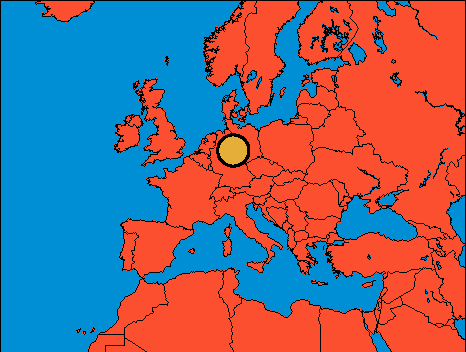
\includegraphics{Figures/approx_size.pdf}
%    \caption{The approximate area of land fertilized by an average single Haber-Bosch plant based on rough estimates above. \hl{Revise as needed based on data estimates.}}
%    \label{fig:map}
%\end{figure}


There are a continuum of options for moving away from this highly centralized scenario. The most extreme alternative would be fully decentralized farm scale fertilizer production, and this would have the largest societal and agricultural impact if deployed in low-income countries where access to fertilizer is limited. There is a large range of farm sizes, but the majority of farms in low-income countries are $\lessapprox$  1 ha \cite{Lowder_2016}. Fertilizer production at the scale of small farms would  correspond to roughly 1 fertilizer production facility per $\sim$1 ha, an increase of $\sim$ 7 orders of magnitude in the total number of fertilizer production facilities. This would also correspond to proportional decrease in the scale of production.
The global average nutrient load needed for fertilization is $\sim$ 50 kg-N/(ha yr) \needcite, which
%\hl{FAO data mch- we may want to round up to 100, based on a discussion with IFDC, I think 50 kg-N/ha is due to disparity}, 
 can be used to estimate the annual budget for on-site fertilizer production based on the cost of fertilizer per country. For example, the price of urea in Ghana in 1999 was one of the highest, approximately \$1100/MT, or \$ 2350/MT-N (urea is 46\% N by weight). \needcite \hl{Would be great to get some more recent numbers here}
 This corresponds to an expected annual fertilizer budget on the order of \$ 120/year. This modest number suggests that decentralized fertilizer production at the scale of small farms must have very low capital and operating costs, even in countries where the cost of fertilizer is very high. Furthermore, the process must be sufficiently robust that specialized operators are not needed for operations or maintenance, and additional constraints such as water usage and fertilization infrastructure (e.g. irrigation) must be considered. However, the current economic situation in many developing countries leads farmers to use little to no fertilizers \needcite, indicating that even the production of an inferior fertilizer product can impact agricultural output if the cost is sufficiently low and infrastructural requirements are minimal. This suggests that ``frugal innovation'' strategies \cite{Weyrauch_2016} may be required for the development of inexpensive and robust processes for producing fertilizer at the scale of small farms in the developing world.
 
An alternative approach to farm-scale production is to target larger farms ($\gtrapprox$ 100 ha), particularly those with irrigation systems in place. These larger farms are more common in developed countries \cite{Lowder_2016}, which presents an economic challenge for decentralized production since it will be competing more directly with traditional fertilizers. For example, the cost of urea in the United States is approximately \$200/MT, or \$435/MT-N as of 2018 \needcite. This is offset by the larger capacity of the farms, and heavier fertilization in the developed countries. Assuming a nutrient load of $\sim$ 100 kg-N/(ha yr) leads to an approximate annual fertilizer production of 10 MT-N/yr budget of $\sim$ \$4,350 per year \hl{It would be even better to get actual numbers for fertilizer budgets for e.g. citrus farms}. This number is relatively modest, but there are additional incentives for larger farms to invest in decentralized fertilization. These larger farms require larger capital investment, and the reduced volatility in price for fertilizers produced on site would improve the predictability of returns. The integration of on-site solar fertilizers with existing irrigation infrastructure may reduce the costs associated with delivering fertilizers to crops, or enable more efficient fertilizer utilization, as discussed further in Sec. \ref{sec:dilute}. There are also challenges for scaling solar fertilizers to larger farms. Solar fertilizer production will require a higher level of technological sophistication, particularly if electrochemical technologies are employed. These approaches will require installation, maintenance, and potentially operation by experts. It is unlikely that a full-time employee could be dedicated to fertilizer production, even at relatively large farms. Nonetheless, periodic access to experts for installation and maintenance is not an issue in developed regions, and numerous industries such as solar capture and home batteries operate on similar business models \needcite. This suggests that solar fertilizers are potentially viable for farm-scale production in developed areas as long as they can be operated with only periodic maintenance.

A third scenario is the production of solar fertilizers at a semi-centralized multi-farm scale. The challenge with more centralized production scenarios is more direct competition with the efficient and inexpensive Haber-Bosch process, since issues with transportation and distribution will be similar. Nonetheless, semi-centralized production can avoid costs and uncertainties associated with international or trans-marine distribution, and the lack of reliance on natural gas as a feedstock can reduce price volatility. Furthermore, coupling solar fertilizer production with the production of other agricultural products such as phosphorus, potassium, agricultural lime, or biochar can alleviate transportation issues by taking advantage of existing infrastructure. For example, a distributed network of fast pyrolysis facilities for simultaneous production of fuel and agricultural biochar has been suggested as a route to carbon-negative energy production \cite{Lehmann2007,Lehmann_2007, Glaser2002}. Coupling these fast pyrolysis plants with photo(electro)chemical nitrogen fixation presents a route to produce nutrient-enriched biochars, as discussed further in Sec. \ref{sec:dilute}. According to a technoeconomic analysis of fast pyrolysis these facilities would process on the order of 2000 MT of biomass per day, with a yield of $\sim$ 20\% biochar  \needcite \hl{https://www.nrel.gov/docs/fy11osti/46586.pdf}. This corresponds to around 150,000 MT-biochar/yr. The amount of biochar applied to farms varies widely from 0.5 - 50 MT/ha \cite{Galinato2011}, but 5 MT/ha is proposed as a reasonable number based on biochar uptake (see Sec. \ref{sec:dilute}) and prior agricultural studies \cite{Galinato2011}. This corresponds to $\sim$ 30,000 ha per facility, or 3000 MT-N/year (assuming 100 kg-N/ha-yr). Assuming the price of nitrogen nutrients is similar to that of urea in the developed world (\$435/MT-N) this leads to a substantial annual budget of \$1.3 million/facility for solar fertilizer production. This would lead to economic viability of more sophisticated solar fertilizer technologies that require full-time expert operation, such as high-temperature operation and/or large-scale solar concentrators. These semi-centralized approaches carry the largest infrastructural burden, and will face substantial challenges in implementation. However, approaches such as enriched biochar production as a byproduct of biofuel present exciting opportunities for simultaneously improving the sustainability of the agricultural and energy sectors through coupled infrastructural developments.

There are many other possible scenarios for solar fertilizer production, and the qualitative analysis above is far from complete. Yet, the order-of-magnitude estimates provided suggest that there are many routes through which solar fertilizers can compete with the established Haber-Bosch process by utilizing the advantages of decentralized production offered by photo(electro)chemical processes. Other niche applications, such as space exploration \cite{Meyer_2016}, may present economic routes to develop solar fertilizer technologies, but likely to be smaller in scale and are beyond the scope of this work. The three scenarios presented here are (1) inexpensive, robust solar fertilizer production at the scale of small farms in remote and undeveloped regions (2) solar fertilizer production integrated with existing infrastructure on larger farms in developed regions, and (3) high-tech solar fertilizer production coupled with production and distribution infrastructure of existing or emerging agricultural products. These scenarios present exciting opportunities to develop scalable decentralized solar fertilizer technologies with the potential for substantial positive impact on society, energy, and the environment.


\subsection{Considerations for dilute fertilizers}
\label{sec:dilute}

The centralized production of fertilizers along with the high purity of Haber-Bosch ammonia has driven the development of solid fertilizers with high weight percent nitrogen (35-85\%) to reduce transportation and storage costs. 
Utilization of solar energy is expected to produce fertilizers with nutrient densities substantially lower than the traditional Haber-Bosch process owing to the lower density of solar energy \cite{MacKay_2013} and the challenges with low efficiency and selectivity in photo(electro)chemical nitrogen fixation \cite{Skulason_2012,Singh_2017}. This is more similar to the biological production of nitrogen that occurs directly in the root system of the plants and results in relatively low local concentrations of fixed N in the soil, approximately 20 kg N/ha yr on average \cite{Smil_1999_2}. As we discuss in Section \ref{sec:targets} the required solar-to-ammonia efficiencies and nutrient concentrations are in principle surprisingly low ($<$1\%); however, these low-concentration fertilizer products differ substantially from existing fertilizers and present a number of challenges as well as some opportunities. Here we consider two varieties of dilute fertilizers: liquid fertilizers in aqueous solutions and solid fertilizers based on carbonaceous materials. These fertilizers have the potential to integrate well with existing agricultural practices, but will also require changes to existing fertilization practices.

Aqueous fertilizers are advantageous since plants require water as well as nutrients, and the process of simultaneously applying fertilizer and water is known as fertigation. Fertigation has formidable potential when coupled with solar fertilizer production since fertigation systems are able to deliver nutrients at a slow rate over time. This leads to a lower overall nutrient concentration relative to solid urea fertilizer, where much of it is washed away. This is particularly effective in areas with high rainfall such as Florida \cite{kadyampakeni_2015}. In tests fertigation has proven to be more effective than both traditional fertilizers and slow release fetilizers in producing growth in citrus trees \cite{Morgan2009}, and leads to higher NO3$^-$ concentrations in the top 15cm of soil \cite{Willis1991}. Tests in peach orchards showed improved fruit sizes with drip fertigation compared to conventional methods \cite{Bryla2005}. These practices may additionally lower by an order of magnitude (down to 13\% of current use) the amount of nitrogen fertilizer needed to achieve the same results as conventional methods \cite{kadyampakeni_2015}. 
Recommended concentrations of nitrogen in fertigation systems range from 50-200 ppm on a mass basis \needcite for most crops. This is in contrast to typical solid urea fertilizers that are 47 wt\%-N. This stark ($\sim$ 4 orders of magnitude) difference in the nutrient density by weight indicates that aqueous dilute fertilizers cannot be economically transported, meaning that aqueous dilute fertilizers are only viable with farm-scale production (see Sec. \ref{sec:decentralized}). This may lead to additional challenges with fertilizer storage, since the solar flux may not always align with crop nutrient needs. This would lead to the need for on-site storage tanks that would increase the footprint of the fertilizer production system, or electrochemical systems that can operate from the electricity grid to produce dilute fertilizers on demand. Another challenge is that fertigation relies on irrigation infrastructure for delivery. This may present a particular challenge for many smallholder farms in sub-Saharan Africa, where only around 7\% \hl{IFDC number from C. Dimkpa} of farms are equipped with irrigation \needcite. Nonetheless, these farms present a sizable initial market, and the prospect of combined fertilization/irrigation systems may be economically viable in already-irrigated farms in the developed world or favor investment in irrigation systems in the developing world.

Another approach to dilute fertilizers is to embed the nutrients with a carrier solid. In most current practical applications the form of nitrogen in fertilizer is urea, which comes as a solid that is dispersed over croplands. Solar fertilizer production could be coupled with adsorbents to uptake and concentrate the products, leading to a solid dilute fertilizer product. In this scenario the ammonia or nitrate products from the photo(electro) chemical reaction could be separated using a solid adsorbent such as activated carbon or biochar \cite{Gon_alves_2011}. This approach is advantageous since application of carbonaceous materials is a common agricultural practice \needcite, and adding adsorbent carbon to soil has been shown to provide many benefits for croplands including water retention, hydraulic conductivity, and resistance to soil erosion \cite{Li2018}. These changes manifest in the form of improved crop production \cite{Glaser2002}, although the magnitude of the improvements depend on the particulars of crop and soil type. Nonetheless, increases of 30\% in seed germination rate and 13\% in biomass production have been observed in woody plants \cite{Chidumayo_1994}. However, implementation of biochar fertilizers may be challenging, since the highest reported ammonia loading for biochar is 16 mg/g of NH$_3$ \cite{Gon_alves_2011}. This translates to 376 mmol/L on a volume basis, and would require 3.8 Mg ha$^-1$yr$^-1$ of activated carbon saturated with ammonia be applied to reach a nutrient loading of 50 kg-N/ha yr. \hl{How does this compare to a typical amount of carbon that would be applied in current agricultural practices?} An additional drawback is that producing high-surface-area carbon requires furnace temperatures above 400 $^\circ$C \cite{Lehmann2007}, which may present an engineering challenge in a low-resource setting. 
%These temperatures would be difficult to achieve without moderate capital investment, and are likely not possible in low resource environments. 
However, in some developed counties biochar facilities have been built and proven profitable \cite{McHenry2009}, and in others would be profitable with a moderate carbon tax \cite{Galinato2011}. This suggests that integration of solar fertilizer facilities with production facilities for carbonaceous soil additives may be a promising strategy, although considerable research is required to determine the efficacy of carbonaceous dilute fertilizers in real agricultural settings.

One enticing possibility for both aqueous and carbonaceous dilute fertilizers is the prospect of improved nutrient management. Currently, the fixed nitrogen in fertilizers is not utilized efficiently, with 20-50\% being lost to leaching or vaporization \cite{Smil_1999_2, Naz_2016}. Leached fertilizer then enters waterways, leading to hypoxic regions in oceans (called dead zones), eutrophication in lakes and rivers, and groundwater contamination \cite{Diaz2008,Conley_2009,Shindo_2006}.  Pollution of this kind is acute in the Gulf of Mexico and the North Sea, due to the intensive agricultural practices of the developed nations upsteam \cite{Diaz2008,Conley_2009}. The vaporization of nitrogen fertilizers can also have deleterious effects on the environment by releasing NO$_x$ compounds, damaging the protective ozone layer \cite{Ravishankara_2009}. The highly concentrated fertilizers responsible for this pollution release nutrients too rapidly for plant uptake, with researchers estimating they are only used at an efficiency of 20-35\% \cite{Naz_2016}. This can have negative effects on the plants themselves, damaging root systems in areas of high concentration \cite{Morgan2009}. The most common strategy for mitigation of these effects is the development of coatings that aid in controlled release of nutrients and enhance uptake efficiency \cite{Naz_2016} \hl{Would be good to get some more examples to cite here}. While these slow-release fertilizers improve performance, the use of dilute fertilizers offers a different approach in which nutrients are delivered at a controlled rate, and in smaller overall amounts \cite{kadyampakeni_2015}. This would enable matching N supply with crop demand. However, substantial additional research into agronomics and plant nutrition is required to determine the potential of this strategy and identify the optimal nutrient concentration and application profile. If dilute fertilizers are applied through fertigation, there is an opportunity to fertilize crops each time they are irrigated, controlling exactly the timing of nitrogen addition. Nitrogen-saturated biochars also hold promise, as these could release nitrogen slowly over a growing season, more effectively resisting leaching than solid urea with the added benefit of improved retention of P and K based fertilizers in the soil through higher ion exchange capacity \cite{Glaser2002}. In addition to improved nutrient management, dilute fertilizers are inherently safer since they will be less corrosive and more difficult to convert into explosives. These factors suggest that further research into the utility and effectiveness of dilute fertilizers is relevant to the field of solar fertilizers.


\section{Solar fertilizer production processes}
\label{sec:approaches}

\subsection{Solar capture, reaction, and separation}


The solar fuels community has identified two basic strategies for conversion of solar to chemical energy: direct capture of photons through photochemistry (photocatlaysis), or indirect capture through photovoltaics coupled to electrochemistry (PV-electrolysis)\cite{McDaniel_2010,Highfield_2015}. Photoelectrochemistry, whereby electrical bias is applied during solar capture represents a third hybrid (indirect+direct) approach for solar-fuel production. There has been considerable debate and analysis regarding the efficiency of each approach for fuel production\cite{Montoya_2017,Daviseaas9793,Lewis_2016,Herron_2015}, and while there is no clear consensus, indirect capture has received considerable attention for the production of hydrogen. This has largely been driven by the goal of achieving solar-to-hydrogen efficiencies which approach 20\% and cost which approach 5.7 \$/kg. 

Some of the same constraints developed in the field of solar-fuels apply to the case of solar fertilizers; however, there are also a number of new considerations which contribute to technological decision making. For instance there are two approaches to make renewable fertilizers. In the first approach, fertilizer manufacturing occurs through a nitrogen reduction process driven (indirectly or directly) by solar energy (renewable ammonia). In the second approach, solar energy drives the production of chemical feedstock’s for the Haber-Bosch process (renewable hydrogen)  (Fig. \ref{fig:reactor}). Another consideration is the low required solar-fertilizer efficiency requirements (when compared with solar-fuels), and the low volatility of products. The final considerations for solar-fertilizers is associated with the desired production location.  While most solar-fuels technologies are envisioned to operate in an industrial setting, there is strong motivation for solar-fertilizers technologies to operate in decentralized locations or at an agricultural site. \hl{While a detailed technoeconomic analysis is beyond the scope of this work, we present some general considerations for each approach.maybe this is misplaced-mch}

\hl{Include a figure here similar to the figures in solar fuels papers (e.g. Nate Lewis' work) comparing these two approaches}
\begin{figure}
    \centering
    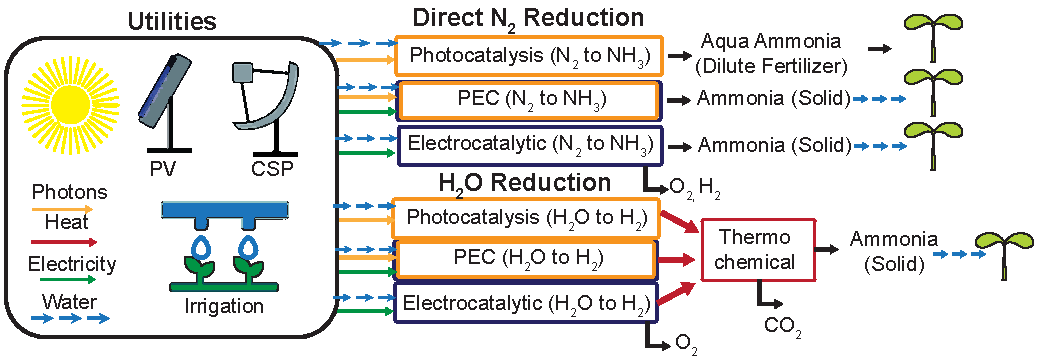
\includegraphics[width=1\textwidth]{Figures/Reactors.pdf}
    \caption{Schematic for solar fertilizer production. Solar fertilizer feedstocks include N\textsubscript{2}, H\textsubscript{2}O or H\textsubscript{2} and solar energy. }
    \label{fig:reactor}
\end{figure}
The direct capture of photons and conversion to fertilizer (renewable ammonia) is the most straightforward route to produce fertilizers at decentralized locations. Direct capture requires the use of a single catalytic material (or composite catalyst). Mass production and distribution of catalyst at low costs is also essential for widespread adoption. It is possible to envision relatively simple reactor designs that integrates directly with an irrigation system. Direct integration within an irrigation system, reduces operational complexity, and costs. These systems must operate without toxic electrolytes, avoiding the need for an additional energy intensive separation processes, and opening the possibility of inexpensive solar fertilizer reactors that could be deployed at the farm scale. However, the concentration of nutrients will be limited by the solar flux, leading to substantial uncertainty and likely lower concentrations (below the desired 1\%). Furthermore, photochemical technologies are relatively untested, and there is currently no catalyst capable of the required solar-to-ammonia efficiency of 0.1 \%. The most widely-used photocatalysts are for environmental applications such as reducing contamination or self-cleaning glass where concentrations are low and catalysts are inexpensive\cite{Bhatkhande_2001,Parkin_2005}. It is possible to envision solar fertilizer schemes that are similar to these environmental applications, but they would likely require close integration with agricultural infrastructure. For example, farms where irrigation is heavily employed are good candidates for direct solar fertilizers, particularly if they are located in remote regions. Roughly 7\% of farms in sub-Saharan Africa make use of irrigation. This is far from a majority, but still represents a substantial agricultural footprint where direct photochemical fertilizers might have a practical impact. \needcite

The alternative approach of capturing solar energy with photovoltaics and subsequently producing electrochemical ammonia also has a number of advantages. Photovoltaic technology is well-established, and efficiencies of 10-20 \% are typical. This leads to a required electrical-to-ammonia efficiency of $\sim$ 1\%, which is relatively low and has been reported at the lab scale for state-of-the-art ammonia electrocatalysts.\cite{Liu2018,Qiu_2018,Song_2018,Zhang_2018,Luo_2018} Furthermore, electrochemical technologies have been demonstrated at scale, including the chloroalkali process, water hydrolysis, and hydrogen fuel cells\cite{Burney1993} \needcite. Electrochemical fertilizer production can be integrated with an electrical grid, providing reliable yields even in periods of no sunlight and the use of high current densities can enable the production of high concentrations of fixed nitrogen. However, large-scale electrochemical processes are far more complex than direct photocatalysis, and may require larger-scale facilities and specialized labor. In addition the practical efficiencies of solar cells on a per-area basis are much lower than their theoretical efficiencies, particularly if they are not installed with advanced technologies such as solar tracking, increasing the capital and labor requirements.\cite{MacKay_2013} Electrochemical processes also require electrolytes to provide electrical conductivity and control the pH. Some reports have indicated that Li-based electrolytes exhibit high performance for electrocatalytic nitrogen reduction to ammonia\cite{Song_2018,Mikosch_2005}. In general the effect of electrolytes on plant growth are unknown, and some electrolytes that contain metals such as Li can be costly, indicating that separation of electrolytes may be required. On the other hand, many electrolytes such as NaCl are abundant and non-toxic, while others such as KOH and Na$_2$H$_2$PO$_4$ could provide an additional source of nutrients if they are not separated. Nonetheless, the need to deal with electrolytes introduces an additional engineering challenge. These intensive production processes would lead to higher capital costs and more centralized production; in this case issues with fertilizer transport would become relevant. As centralization increases the process will be in more direct competition with the established Haber-Bosch process, and more detailed technoeconomics will be necessary to determine if such an approach is competitive. Nonetheless, the scale of electro-chemical processes is still expected to be orders of magnitude below Haber-Bosch, and the process is likely to be less capital-intensive and more robust to uncertainty in electrical power. This suggests that agricultural areas in developed countries, near medium or large cities, or in land-locked areas are most promising for indirect capture of solar energy and subsequent electro-chemical conversion to fertilizers.

\hl{Add a table here with properties/advantages/disadvantages of direct vs. indirect?}

\subsection{Proposed process designs}

\begin{figure}
    \centering
    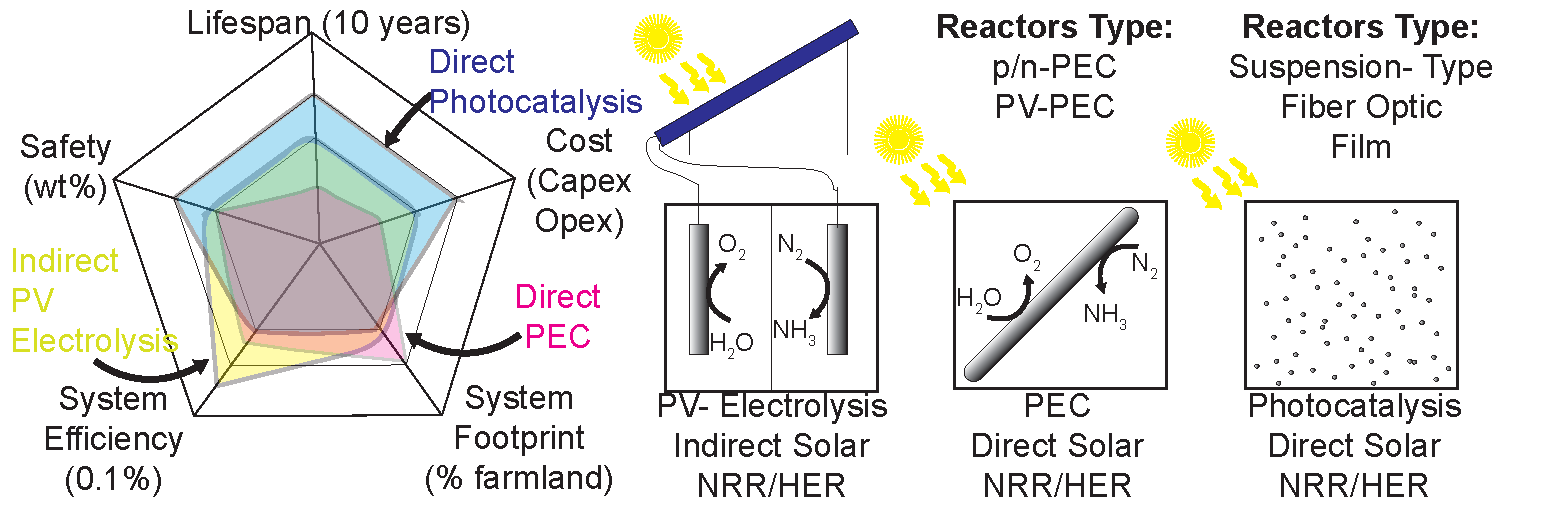
\includegraphics[width=1\textwidth]{Figures/Systems.pdf}
    \caption{}
    \label{fig:systems}
\end{figure}

 Briefly below we outline potential system architectures for solar-fertilizers, with an emphasis on discerning their cost (capitol and operational), efficiency, safety, and size.

\subsection*{Direct approaches for solar-fertilizers}

While there are currently no photocatalytic chemical production processes operation at scale, there exists a strong literature on photochemical reactor design for environmental applications and solar-fuel production.\cite{Mckone_2013,Birnie2006,walter_2010} It is likely, that the same principles and strategies will apply to the production of solar fertilizers. One reactor type heavily investigated is the suspension type reactor. A notable challenge with suspension type particles is the mixing of reduced and oxidized species (oxygen, ammonia and hydrogen), and the need to separate the two gas phase species. Despite these challenges, it is projected to be the cheapest approach to solar-fuel production.  In addition, there are  The first requirement of a photocatalytic reactor is to have an immobilized photocatalyst over which fluid can flow to prevent loss of catalyst. In practice, the photocatalyst is applied as a coating on a transparent material. Two common designs in commercial applications are flat plates\cite{Brandi_1999} and fiber glass cloths\cite{Horikoshi_2002} coated in photocatalyst. Reactors involving honeycombs of catalyst with embedded optical fibers to convey light have been proposed for CO$_2$ reduction photocatalysis.\cite{Ola_2015} These are all viable in principle for N$_2$ reduction, though capital costs and durability may be factors in the eventual viability of a given design.

Due to the low rates of reaction in current generation photocatalysts, a successful reactor design will likely be either a stagnant tank solar collection system or a low flow reactor, similar to a continuously stirred tank reactor (CSTR.) The photocatalyst could be either immersed in water or suspended above water to perform the reaction in an aqueous phase or gas phase respectively. The produced ammonia be kept at a high concentration within the reactor to maintain a high product concentration. In the case of using activated carbon as an adsorbent, the carbon would be suspended above the liquid to allow the gaseous products to diffuse into the pores in the gas phase.

Coupled solar capture/electrocatalysis systems are able to be more centralized than their photchemical analogs. A standard system may look similar to a membrane reactor from a chloralkali process, with flow cells consisting of electrodes separated by a semi-permeable membrane arranged in arrays.\cite{} These would be positioned near solar farms in rural areas. These could produce an aqueous solution of ammonia, which would be delivered in pipelines or by truck to nearby farms. Another possibility is coupling a biochar production facility with an electrochemical nitrogen system. The ammonia could be produced and concentrated in a bed of biochar. The biochar would then be delivered to local farms via truck or rail connections to be applied as fertilizer. Given that biochar facilities are already economically promising, the latter option may prove exceptionally attractive.\cite{Galinato2011}

\subsection*{Indirect approaches for solar-fertilizers (Photovoltaic-Electrolysis)}

Coupled Photovoltaic/electrochemical systems are currently more efficient than the photochemical approaches. However, some of the common reactor configurations require higher initial capital investment than photochemical approaches, due to the cost of the reactor components (membranes and catalysts). Electrolysis systems may be promising for use in small/medium ammonia manufacturing plants in a semi-decentralized manufacturing model. The largest challenge with the electrolysis systems is that there are no selective catalysts capable of reducing dinitrogen. The three prominent approaches which could be employed include alkaline based electrolyzer, proton exchange membrane (PEM) electrolyzer, and solid oxide based electrolysis (SOEC). 

\todo{need appropriate citations}Alkaline electrolysis cells operate in with a basic electrolyte (usually KOH or NaOH), and have achieved achieved efficiency's of 50\%-60\% and current densities of 100-300 mA/cm$^2$ for hydrogen production. PEM electrolyzers use a polymer membrane (Nafion) as a solid electrolyte, and have demonstrated efficiencies between 55\% and 70\% and current densities higher than 1600 mA/cm$^2$. And solid oxide electrolysis (SOECs) which operate in the mid temperature range (100-200 $^\circ$C) are able to achieve higher efficiencies (85\%-90\%). Unfortunately, the performance of current state of the art electrolysis cells do not translate to nitrogen reduction based electrolysis systems. 

The materials used in these reactors are costly because of the high temperatures that have to be withstood during the reaction. The biggest issue with SOECs is that the technology is still in early stages of development and sealing and corrosion problems are common. Due to the high initial capital investment, high efficiency, and high temperatures these reactors would be best used in large scale plants. 

\section{Preliminary Performance Targets}
\label{sec:targets}

There has been a substantial recent increase in photo(electro)chemical nitrogen fixation research, yet there are no targets for how efficient these processes need to be. In this section we briefly outline targets for solar-to-ammonia efficiency, total fixed nitrogen concentration, and required rates of nitrogen fixation that have the potential to enable solar fertilizer production. These targets are not meant to be authoritative, but rather provide guidelines for catalyst development and fertilizer testing. 

One key consideration is the overall efficiency required to convert solar energy to fertilizer. First, we estimate the areal energy density required for fertilization based on an assumption of 50 kg-N/(ha yr) provided by ammonia-based fertilizers:
\begin{equation}
\mathrm{
50 \frac{kg_N}{ha . yr} \times \frac{10^3}{14} \frac{mol_{NH_3}}{kg_N} \times \frac{667}{2} \frac{kJ}{mol_{NH_3}} \times \frac{1}{10^4} \frac{ha}{m^2} \times \frac{1}{3.15e7} \frac{yr}{s} = 3.77 \frac{mW}{m^2}
}
\end{equation}
%this remarkably low energy density is roughly 6 orders of magnitude below the solar constant of 1000 W/m$^2$, indicating that high efficiencies are not necessary. 
An initial estimate of necessary efficiency can be obtained by assuming 8 hours of full sunlight per day and 1\% of arable land dedicated to solar capture \cite{Medford_2017}. In this case the average solar flux is 333 W/m$^2$ and the corresponding required solar-to-ammonia efficiency is $\sim$0.1 \%. Data on actual average solar fluxes reveals that they vary from 120 - 280 W/m$^2$ depending on latitude \cite{MacKay_2013}, and there is also considerable variability in the nutrient load required, ranging from 15-200 kg-N/m$^2$ depending on a myriad of factors including crop and soil type \needcite. Based on these estimates the required solar-to-ammonia efficiency may range from 0.05 - 1.25 \% depending on solar flux and required nutrient load. These estimates assume that 1\% of arable land is dedicated to solar capture, and will vary linearly with the percentage of land available. We propose that 1\% is a relatively conservative number, corresponding to 100 m$^2$/ha or roughly 6 typical solar panels per hectare \needcite. Notably, solar-to-ammonia efficiencies as high as 0.02 \% have been reported for nitrogen fixation photocatalysts, suggesting that the efficiency target is feasible with further research.\cite{Hirakawa_2017} \needcite

In addition to efficiency it is also critical to consider the concentration of fixed nitrogen needed for a product to be considered a fertilizer. The limiting case can be determined by assuming that the nutrients will be included directly in the irrigation lines. However, the amount of irrigation needed is highly variable depending on crops, rainfall, location, and socioeconomic factors (http://www.fao.org/docrep/u5835e/u5835e04.htm). Nonetheless, we propose an estimate of 1500 L/ha/y as a typical number for practical scenarios. Further, we note that while 50 kg-N/(ha yr) is a typical nitrogen nutrient load, the critical lower boundary for nutrient consumption can be as low as 15 kg-N/(ha yr). From these estimates we propose a lower boundary of 1 kg-N/L, or 1 wt \% N, as a convenient estimate for the minimum nitrogen concentration that can be considered a fertilizer \hl{compare to aqua ammonia and potential get insight from IFDC on what the potential impact might be of these low loads. Any previous experience where aqua ammonia is used for direct application?}. This is roughly 1 order of magnitude lower than existing aqueous fertilizers, but it is 5-8 orders of magnitude above the concentrations reported for typical photo(electro)chemical nitrogen fixation processes where yields are typically reported in units of $\mu$M or mM. This large gap between the proximity of efficiency and concentration targets is due to a combination of large water volumes and the short testing times that are typically employed for photo(electro)catalysts. Photocatalytic ammonia production is often measured in the gas-phase, where ammonia sticks to the catalyst surface and must be removed through water or heat, leading to low concentrations, and in aqueous photo(electro)chemical settings the fluid volumes are typically on the order of 100mL while illumination areas are on the order of cm$^2$. Furthermore, testing times on the order of days to weeks are considered long by academic standards. This leads to extremely low concentrations that are outside of the regime that can be considered fertilizer. Operating the catalysts in higher ammonia concentration regimes may impact the performance of the process, suggesting that future efforts should focus on designing cells and testing procedures that lead to substantially higher concentrations. These higher concentrations lead to an additional advantage for analytical characterization, since difficulties in quantifying ammonia at nM - $\mu$M concentrations have plagued the field. As concentration increases the issues with contamination will be less prevalent, and the presence of ammonia should become unmistakable due to its pungent odor that can be detected with concentrations of about 50 ppm\cite{Leonardos_1969} (equivalent to 3 mM in the aqueous phase).

A further consideration that is particularly relevant to electrochemical ammonia production is the current densities that are required for practical operation. In the case of solar fuels the overpotential for oxygen evolution has been defined as the potential at which the current is equal to 10 mA/cm$^2$, equivalent to 10 \% solar-to-fuel efficiency. In the case of solar fertilizers the necessary current will be substantially lower, due to the substantially lower solar-to-ammonia efficiency requirements. For simplicity, we will assume that a 0.1\% solar-to-ammonia efficiency is required. However, an additional consideration that is more relevant for electrochemical nitrogen fixation is the Faradaic efficiency that governs the selectivity to ammonia (or nitrates) over other possible products. Indeed, low selectivity to ammonia due to hydrogen evolution has proven to be a critical challenge for electrochemical ammonia synthesis.\cite{Singh_2017} Typical reported ammonia selectivities are $<$ 1\%, although several recent reports have achieved Faradaic efficiencies on the order of 10 \%. By assuming 10 \% Faradaic efficiency and an overall solar-to-ammonia efficiency of 0.1 \%, the relevant current density is 1 mA/cm$^2$. Notably, Faradaic efficiency is often a strong function of applied potential (and the resulting current density) \needcite, with high Faradaic efficiencies typically corresponding to very low current densities on the order of nA/cm$^2$ - $\mu$A/cm$^2$. Nonetheless, a recently-reported carbon-based catalyst achieved $>$10 \% Faradaic efficiency at a current density of ca. 4 mA/cm$^2$ \needcite, indicating that it is possible to achieve high Faradaic efficiencies at the proposed operating current of 1 mA/cm$^2$. Measuring overpotential and Faradaic efficiencies at practical current densities provides a useful route to identifying electrocatalysts that are promising for solar fertilizer production.

\hl{Possible paragraph or table outlining suggested testing standards (temperature, pressure, pH, illumination intensity, etc.) for photo- and electrochemical approaches?}



\section{Conclusions}

Solar fertilzers present an exciting opportunity to directly capture diffuse solar energy and convert it to chemical energy that can be applied at or near the point of production. The technology falls at the complex nexus of energy and agriculture, and substantial additional research is needed to establish the most promising approaches and demonstrate the technology. This work grapples with some initial considerations from the perspective of agronomics and photoelectrochemistry, and identifies some preliminary metrics that will aid in the development and deployment of solar fertilizer technologies. Specific metrics are presented to identify the target solar-to-ammonia efficiency (0.1\%), minimum nitrogen concentration (1 wt\%), and electrochemical current density (1 mA/cm$^2$) that may enable solar fertilizer technology, and considerations for assessing direct and indirect capture and conversion of solar energy are presented. The metrics and considerations presented draw on a range of expertise in the diverse fields of agronomics, photoelectrocatalysis, and process systems engineering, and provide a starting point for further development of solar fertilizer technologies. There are many possible routes forward for this nascent field, and identifying the most promising will require a diverse range of technical, social, and economic considerations. However, the vast potential impact of solar fertilizers on the growing problem of world hunger makes this challenging endeavor worthwhile.


